\documentclass{beamer}

\usepackage[utf8]{inputenc}
\usepackage{default}
\usepackage{multirow}

\title{Evaluating Feasibility of Container Virtualization for Virtual Network Functions}
\subtitle{M.S Thesis Defense}
\institute{Galatasaray University}
\author{Uğurcan Ergün \\ Advisor: Dr. Atay Özgövde}
\date{4 July 2018}

\begin{document}

\begin{frame}
  \titlepage
\end{frame}

\begin{frame}{Agenda}
 \begin{itemize}
  \item Problem
  \item Motivation
  \item Literature Review
  \item Methodology
  \item Results
  \item Conclusion
 \end{itemize}
\end{frame}

\begin{frame}{Problem}
 \begin{itemize}
  \item Network operators starting to experience unprecedented levels of mobile data usage and
network traffic.
 \item There are certain limitations that constrain them when trying to improve the infrastructure.
 \item They pursue to implement dynamic, flexible networks with various new technologies.
 \item Design of 5G networks implies that telecom operators are trying to approximate telecom
 infrastructure to cloud infrastructure
 \end{itemize}

\end{frame}

\begin{frame}{Problem}
 \begin{itemize}
  \item Computers networks are still complex and hard to manage because of the proprietary and tightly
coupled nature of the most network devices.
  \item Software defined networking try to implement the lessons learned in virtualization to the networks.
  \item But there are still significant amount of proprietary network appliances.
  \item Network function virtualization has been introduced as a solution
 \end{itemize}

\end{frame}

\begin{frame}{Motivation}
 \begin{itemize}
  \item Companies that rely on cloud computing started using a different way to use software on the cloud.
  \item Decoupling software into independent services and running them inside a new
  virtualization solution called containers.
  \item We believe this client native approach to software and performance benefits of containers can be used
  to utilize network function virtualization better.
 \end{itemize}

\end{frame}

\begin{frame}{Literature Review}
 \begin{itemize}
  \item Most of the works in the literature are focused on implementing network function virtualization with
  standard hypervisor virtualization.
  \item For infrastructure cloud platform Openstack seems to be a de-facto choice as it also has an NFV project.
  \item Few works that implemented VNFs with containers were focused on different areas such as edge computing.
 \end{itemize}

\end{frame}


\begin{frame}{Methodology}{Setup}
 \begin{itemize}
  \item Our focus would be measuring network performance for Kubernetes.
  \item We installed a Kubernetes cluster in a desktop computer.
  \item We picked nginx that can function as a simple network function for experiments.
  \item We used Kubernetes deployments for managing containers on the cluster.
 \end{itemize}
\end{frame}

\begin{frame}{Methodology}{Kubernetes Architecture}
  \begin{center}
   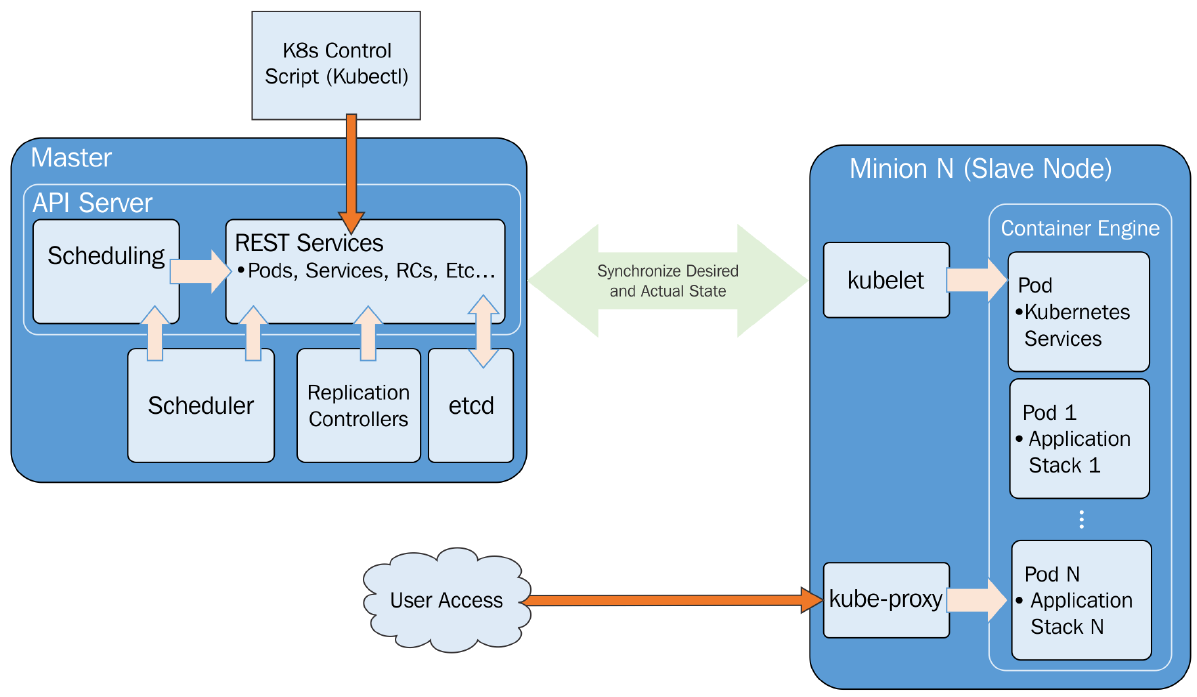
\includegraphics[height=7cm, width=10cm]{figures/k8s.png}
  \end{center}
\end{frame}

\begin{frame}{Methodology}{Kubernetes Networking}
  \begin{center}
   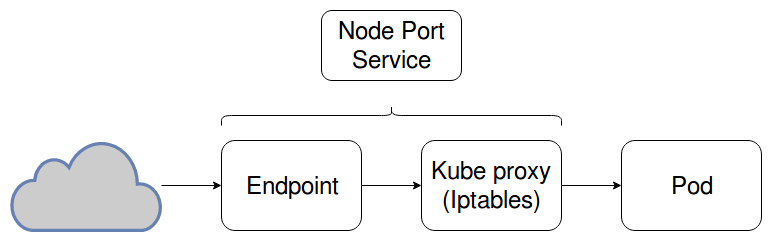
\includegraphics[height=4cm, width=10cm]{figures/conn.png}
  \end{center}
\end{frame}

\begin{frame}{Methodology}{Experiment Design}
 \begin{itemize}
  \item Experiment cases include different configuration of containers with different
  resource limits and instance counts.
  \item These experiments then run with automated scripts using an open source load testing tool vegeta.
  \item Network latency is then reported as mean, maximum and different percentile values.
  \item Each experiment has been run 10 times and then averaged.
 \end{itemize}
\end{frame}

\begin{frame}{Methodology}{Percentile Metrics}
 \begin{itemize}
  \item Percentile metrics are used for getting more accurate information about the application performance.
  \item They aren't affected by outlier data points contrary to arithmetic means.
 \end{itemize}
 \begin{block}{Calculation of percentile metrics}
  First the results are sorted from minimum to maximum and then highest 100-n percent of the results are deleted.
  The maximum remaining result is called the nth percentile result.
 \end{block}
\end{frame}

\begin{frame}{Results}{First Experiment: Configuration}
  \begin{table}[h]
    \caption{Number of instances for each deployment}
    \centering
    \begin{tabular}{ccc}
    Deployment 1 & Deployment 2 & Deployment 3 \\
    \hline
    1 & 1 & 1 \\
    5 & 5 & 1 \\
    10 & 1 & 1 \\
    12 & 12 & 1 \\
    25 & 1 & 1 \\
    25 & 25 & 1 \\
    37 & 37 & 1 \\
    50 & 1 & 1 \\
    50 & 50 & 1 \\
    75 & 1 & 1 \\
    100 & 1 & 1 \\
    \hline
    \end{tabular}
  \end{table}
\end{frame}

\begin{frame}{Results}{First Experiment}
  \begin{center}
   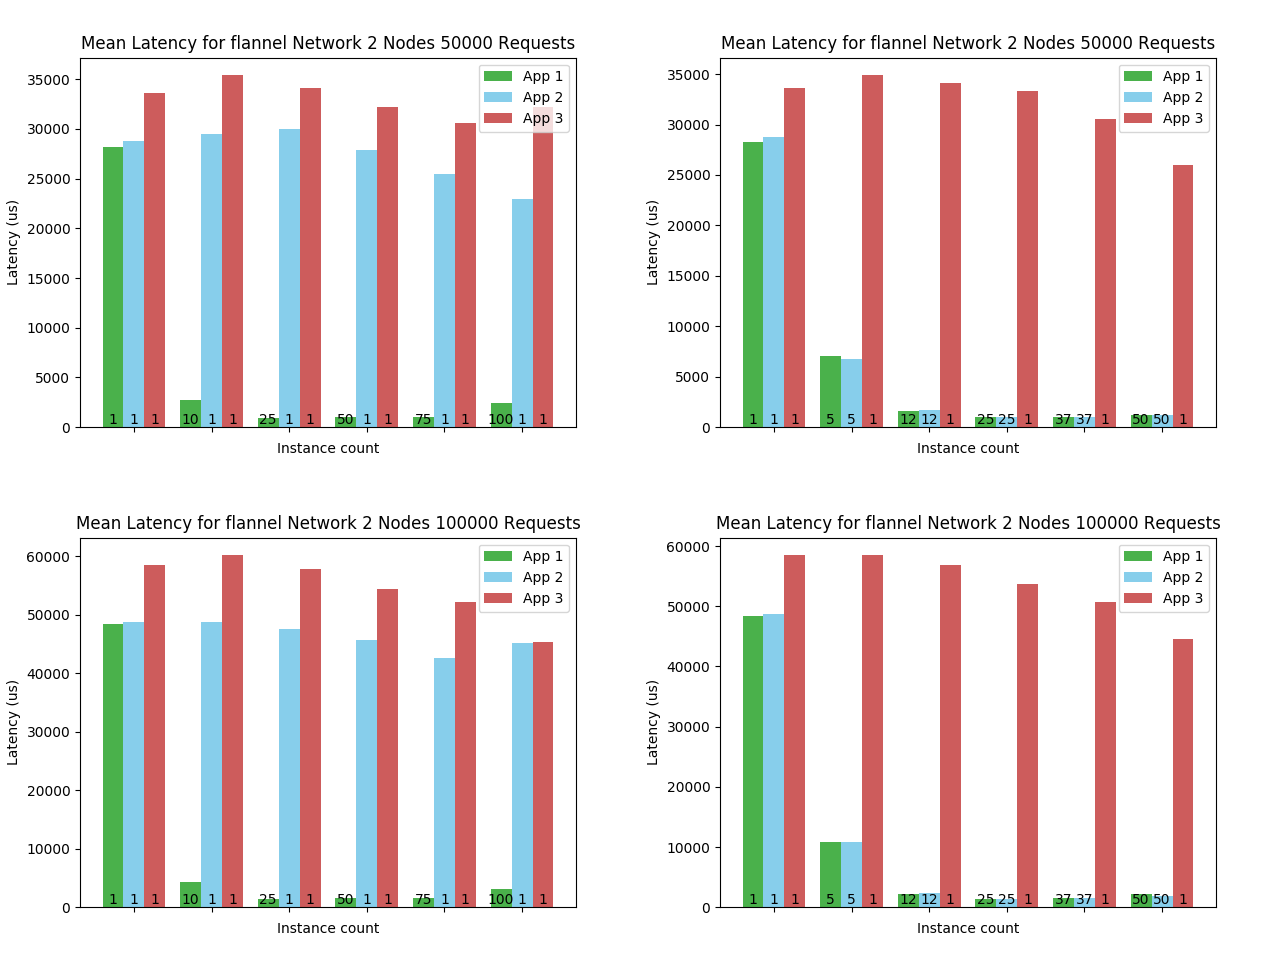
\includegraphics[height=7cm, width=9cm]{figures/flannel.png}
  \end{center}
\end{frame}

\begin{frame}{Results}{First Experiment: Discussion}
 \begin{itemize}
  \item Even an aged desktop computer can run high number of containers.
  \item Computer might support more 100 containers.
  \item Applications doesn't seem to affected from co-location related latency.
  \item Slight amount of increase at the final steps latencies are caused by host load
 \end{itemize}
\end{frame}

\begin{frame}{Results}{Second Experiment: Configuration}
\begin{table}[h]
\centering
\begin{tabular}{ |l|l|l| }
\hline
Setup & Left side & Right side \\ \hline
Setup A &  ~~5 *  250m & ~~5 *  250m \\
Setup B & 10 *  250m &  20 *  250m \\
Setup C &  1 * 1250m &   1 * 2500m \\
Setup D &  1 * 2500m &   1 * 5000m \\ \hline
\multirow{3}{*}{Setup E} 
 & 10 *  125m & 20 *  125m \\
 &  ~~5 *  250m & 10 *  250m \\
 &  ~~3 *  500m & ~~5 *  500m \\ \hline
\multirow{3}{*}{Setup F}
 & 20 *  125m & 40 *  125m \\
 & 10 *  250m & 20 *  250m \\
 &  ~~5 *  500m & 10 *  500m \\ \hline
\end{tabular}
\caption{experiment setups as instance count * CPU limits}
\end{table}
\end{frame}


\begin{frame}{Results}{Second Experiment: Setup A}
  \begin{center}
   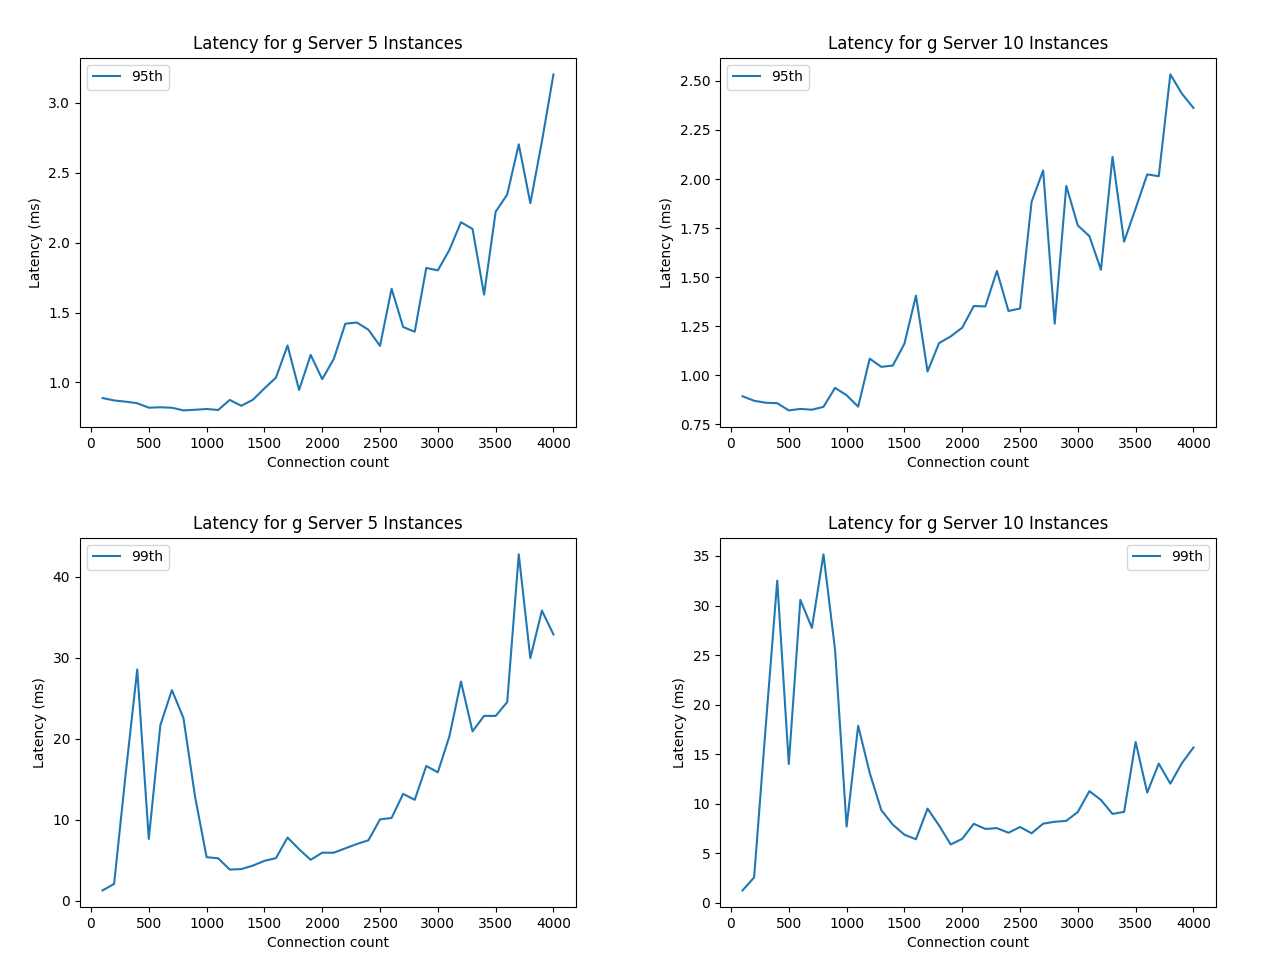
\includegraphics[height=7cm, width=9cm]{figures/g5_10.png}
  \end{center}
\end{frame}

\begin{frame}{Results}{Second Experiment: Setup B}
  \begin{center}
   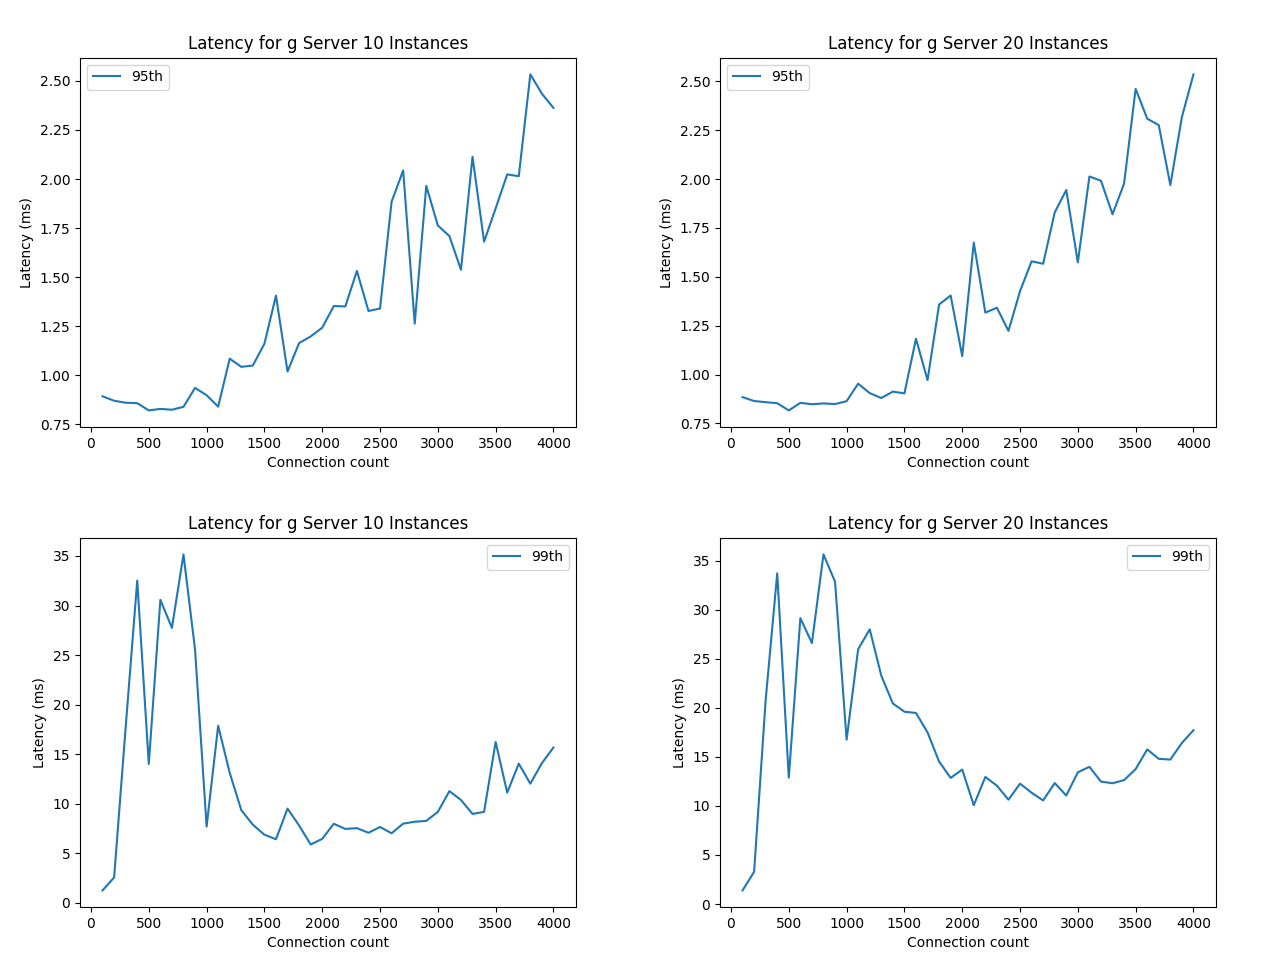
\includegraphics[height=7cm, width=9cm]{figures/g10_20.png}
  \end{center}
\end{frame}

\begin{frame}{Results}{Second Experiment: Setup C}
  \begin{center}
   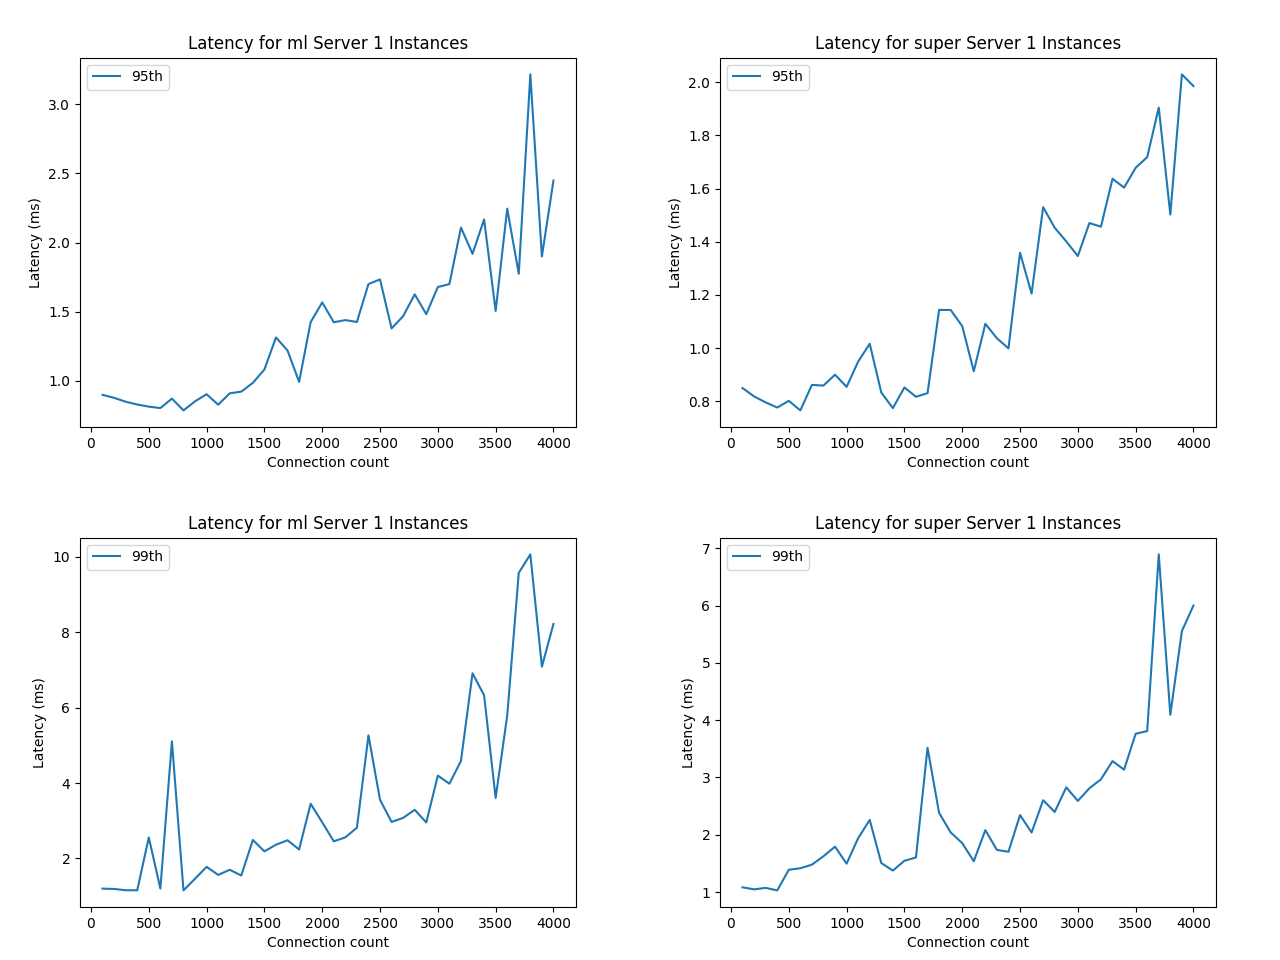
\includegraphics[height=7cm, width=9cm]{figures/ml1_super1.png}
  \end{center}
\end{frame}

\begin{frame}{Results}{Second Experiment: Setup D}
  \begin{center}
   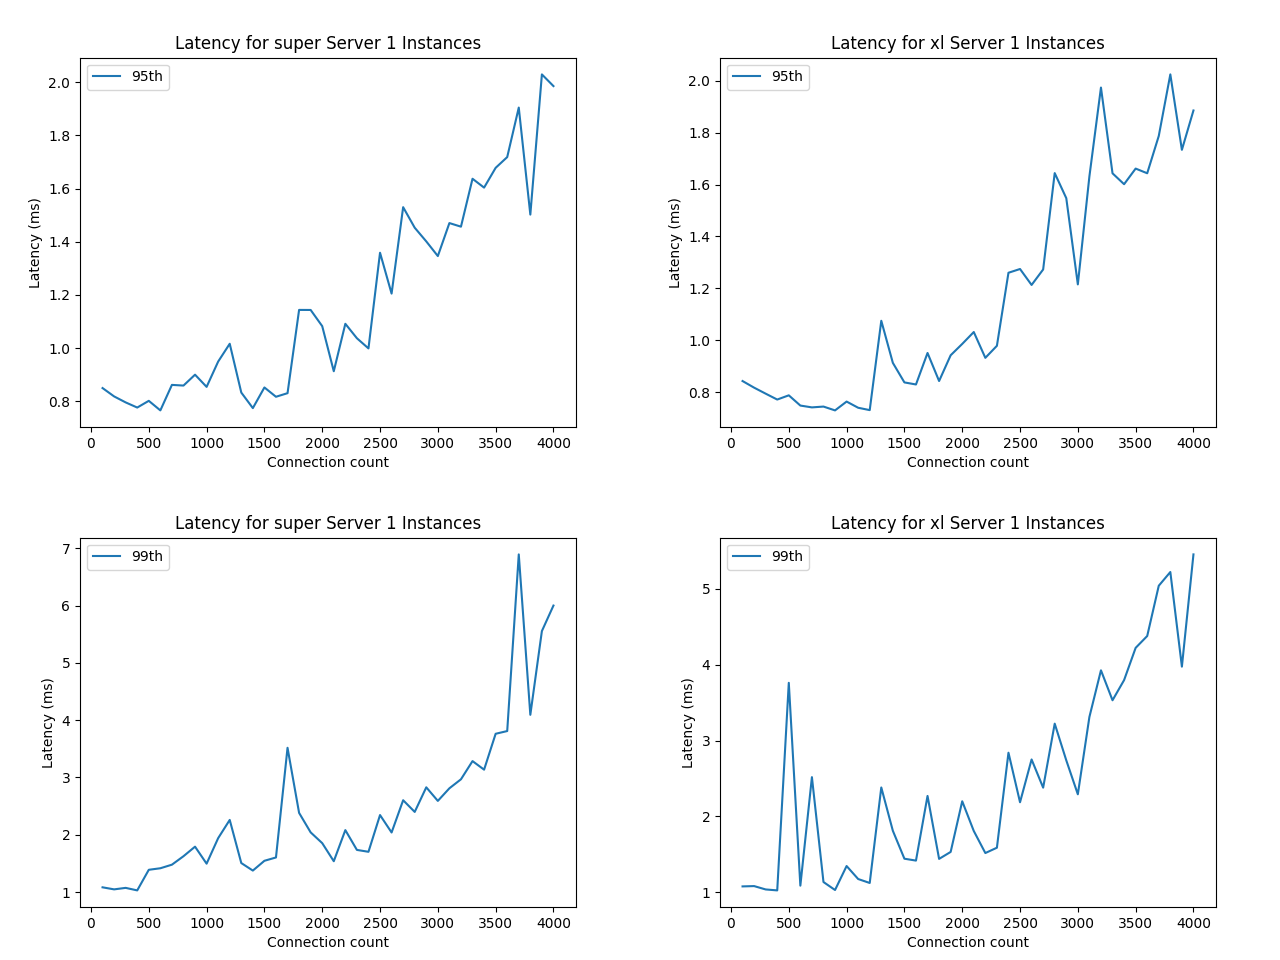
\includegraphics[height=7cm, width=9cm]{figures/super1_xl1.png}
  \end{center}
\end{frame}

\begin{frame}{Results}{Second Experiment: Setup E}
  \begin{center}
   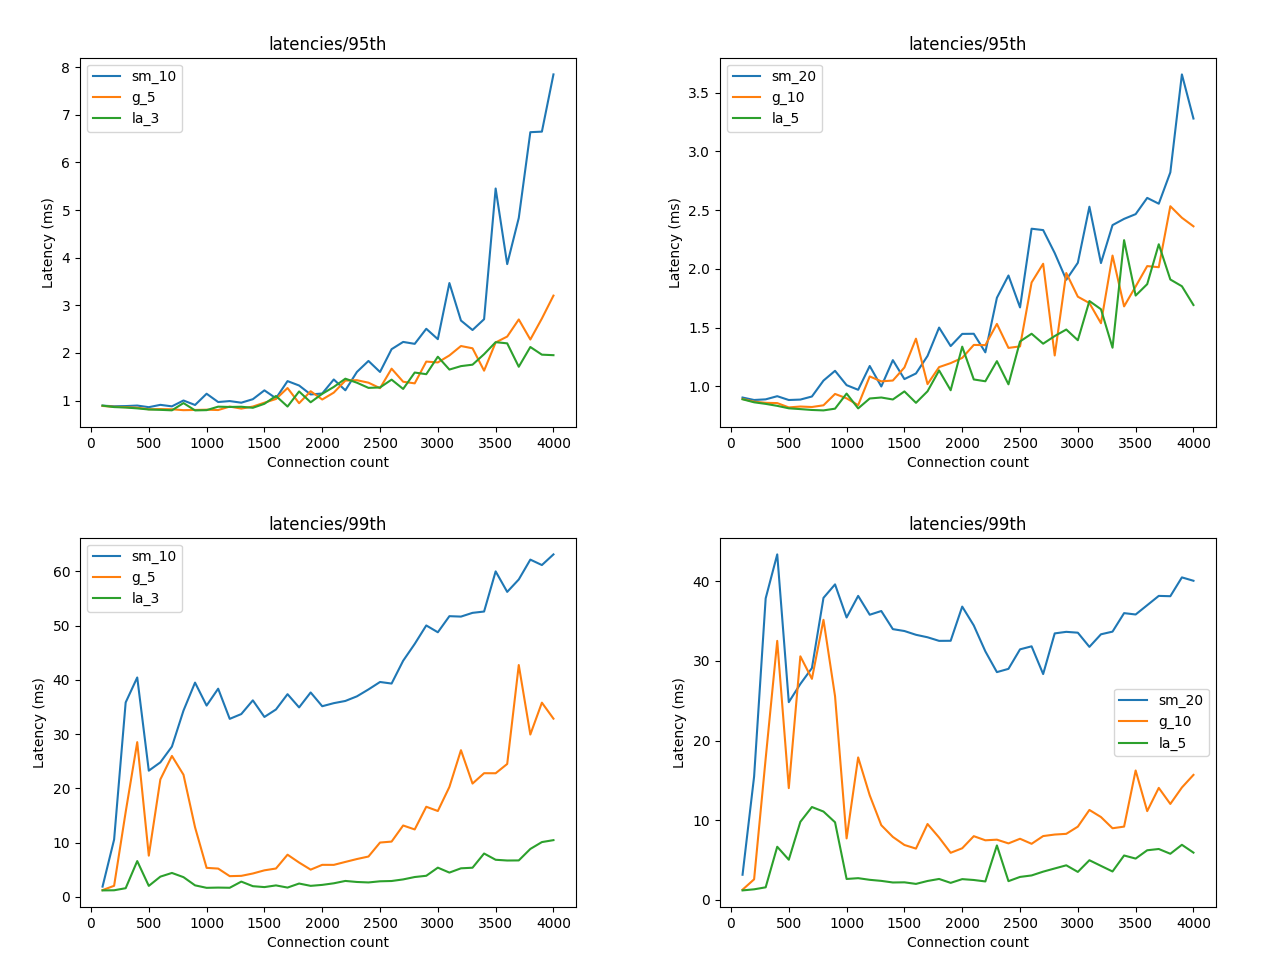
\includegraphics[height=7cm, width=9cm]{figures/multi1250_2500.png}
  \end{center}
\end{frame}

\begin{frame}{Results}{Second Experiment: Setup F}
  \begin{center}
   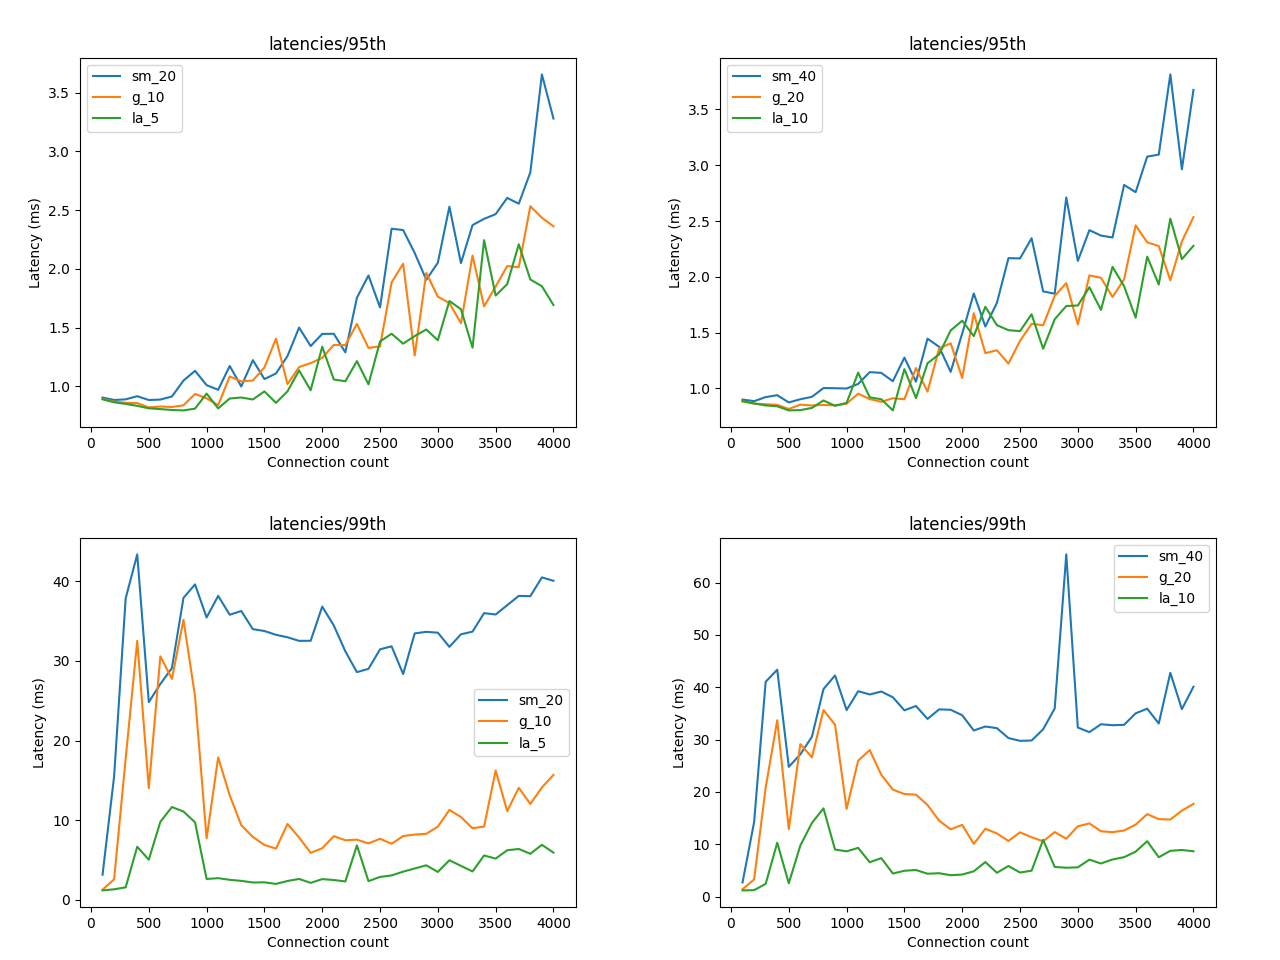
\includegraphics[height=7cm, width=9cm]{figures/multi2500_5000.png}
  \end{center}
\end{frame}

\begin{frame}{Results}{Second Experiment: Discussion}
 \begin{itemize}
  \item Using multiple containers instead of a single one increases overhead. But
  some cases perform very similarly
  \item Major differences in latencies mostly occur in slowest 5 percent of connections.
  \item Balance between instance count and resource limit proves crucial for performance.
  \item After a certain point extra instances started to add more overhead.
 \end{itemize}
\end{frame}

\begin{frame}{Conclusions}
 \begin{itemize}
  \item Fundamental technologies for implementing virtual network functions are
  present in container environments.
  \item Even for a very small percent of results there is significant peaks in latency. This
  may not acceptable for some network functions.
  \item As a solution specialized high speed networking software may be needed.
  \item There are still no out of box solutions for network functions in container platforms.
 \end{itemize}

\end{frame}


\begin{frame}
 \begin{center}
 \Huge Thank you for listening
 \end{center}
\end{frame}

\begin{frame}
 \begin{center}
 \Huge Questions ?
 \end{center}
\end{frame}

\end{document}
